\begingroup
% https://tex.stackexchange.com/questions/670034/centering-tikzpicture-in-tabularray/670036#670036
\tikzset{baseshift/.style={yshift=-\the\dimexpr\fontdimen22\textfont2}}
\tikzset{every picture/.style={scale=0.6, baseline={([baseshift]current bounding box.center)}}}

\begin{table}[h!]
    \centering
    \SetTblrInner{rowsep=3pt}
    \def\colplot{cyan}
    \def\a{-0.3}
    \def\b{3.8}
    \def\xmin{-0.1}
    \def\xmax{4.1}
    \def\amp{1}
    \def\puls{8}
    \def\damp{0.6}
    \def\samp{200}
    \begin{tblr}{
        vspan=even, hspan=minimal,
        colspec={| Q[c] Q[c] | Q[c] Q[c] |}, rowspec={Q[m] Q[m] Q[m] Q[m] Q[m] Q[m] Q[m]}
    }
        \hline
        $f(t) \mathbf{1}_{t > 0}$ & $f(t)$ & $\mathcal{L}(f)(p)$ & \\ \hline\hline
        % Row 2
            \begin{tikzpicture}
                \draw[-latex] (\xmin,0) -- (\xmax,0);
                \draw[-latex] (0,-0.2) -- (0,1.5);
                \draw[\colplot, thick, domain=\a:0] plot (\x, 0);
                \draw[\colplot, thick] (0,0) -- (0,1) -- (\b,1);
            \end{tikzpicture}%

        & $ A $ & $\displaystyle \frac{A}{p} $ & 

            \begin{tikzpicture}
                \draw[-latex] (\xmin,0) -- (\xmax,0);
                \draw[-latex] (0,-0.2) -- (0,1.5);
                \draw[\colplot, thick, domain=1/6:\b, samples=\samp] plot (\x, {1/(6*\x)});
            \end{tikzpicture}%

        \\ \hline

        % Row 3
            \begin{tikzpicture}
                \draw[-latex] (\xmin,0) -- (\xmax,0);
                \draw[-latex] (0,-0.2) -- (0,1.5);
                \draw[\colplot, thick, domain=\a:0] plot (\x, 0);
                \draw[\colplot, thick] (0,0) -- (\b,1);
            \end{tikzpicture}%

        & $ a\,t$ % \cdot u(t) $ 
        & $\displaystyle \frac{a}{p^2} $ & 
        % \adjustbox{valign=c}{%
            \begin{tikzpicture}
                \draw[-latex] (\xmin,0) -- (\xmax,0);
                \draw[-latex] (0,-0.2) -- (0,1.5);
                \draw[\colplot, thick, domain=0.40824829046:\b, samples=\samp] plot (\x, {1/(6*\x^2)});
            \end{tikzpicture}%

        \\ \hline

        % Row 4
            \begin{tikzpicture}
                \draw[-latex] (\xmin,0) -- (\xmax,0);
                \draw[-latex] (0,-0.2) -- (0,1.5);
                \draw[\colplot, thick, domain=\a:0] plot (\x, 0);
                \draw[\colplot, thick] (0,0) -- (0,\amp);
                \draw[\colplot, thick, domain=0:\b] plot (\x, {\amp*exp(-\damp*\x)});
            \end{tikzpicture}%

        & $ \mathrm{e}^{-at}$ % $ \cdot u(t) $ 
        & $\displaystyle \frac{1}{p + a} $ & 
            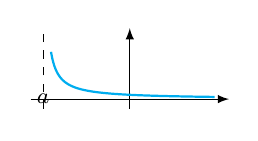
\begin{tikzpicture}
                \draw[-latex] (\xmin,0) -- (\xmax,0);
                \draw[-latex] (2,-0.2) -- (2,1.5);
                \draw[dashed] (1/6,-0.2) -- (1/6,1.5);
                \node at (1/6, 0) {\footnotesize $a$};
                \draw[\colplot, thick, domain=1/3:\b, samples=\samp] plot (\x, {1/(6*(\x-1/6))});
            \end{tikzpicture}%
            
        \\ \hline

        % Row 5
            \begin{tikzpicture}
                \draw[-latex] (\xmin,0) -- (\xmax,0);
                \draw[-latex] (0,-0.2) -- (0,1.5);
                \draw[\colplot, thick, domain=\a:0] plot (\x, 0);
                \draw[\colplot, thick, domain=0:\b, samples=\samp] plot (\x, {5*\x*exp(-1.5*\x)});
            \end{tikzpicture}%

        & $ t\, \mathrm{e}^{-at}$ % $ \cdot u(t) $ 
        & $\displaystyle \frac{1}{(p + a)^2} $ & 
            \begin{tikzpicture}
                \draw[-latex] (\xmin,0) -- (\xmax,0);
                \draw[-latex] (0,-0.2) -- (0,1.5);
            \end{tikzpicture}%

        \\ \hline

        % Row 6
            \begin{tikzpicture}
                \draw[-latex] (\xmin,0) -- (\xmax,0);
                \draw[-latex] (0,-0.65) -- (0,1.05);
                \draw[\colplot, thick, domain=\a:0] plot (\x, 0);
                \draw[\colplot, thick, domain=0:\b, samples=\samp] plot (\x, {\amp/1.5*sin(\puls*\x r)});
            \end{tikzpicture}%

        & $ \sin(\omega t)$ % $ \cdot u(t) $ 
        & $\displaystyle \frac{\omega}{p^2 + \omega^2} $ & 
            \begin{tikzpicture}
                \draw[-latex] (\xmin,0) -- (\xmax,0);
                \draw[-latex] (0,-0.65) -- (0,1.05);
            \end{tikzpicture}%

        \\ \hline

        % Row 7
            \begin{tikzpicture}
                \draw[-latex] (\xmin,0) -- (\xmax,0);
                \draw[-latex] (0,-0.65) -- (0,1.05);
                \draw[\colplot, thick, domain=\a:0] plot (\x, 0);
                \draw[\colplot, thick] (0,0) -- (0,\amp/1.5);
                \draw[\colplot, thick, domain=0:\b, samples=\samp] plot (\x, {\amp/1.5*cos(\puls*\x r)});
            \end{tikzpicture}%

        & $ \cos(\omega t)$ % $ \cdot u(t) $ 
        & $\displaystyle \frac{p}{p^2 + \omega^2} $ & 

            \begin{tikzpicture}
                \draw[-latex] (\xmin,0) -- (\xmax,0);
                \draw[-latex] (0,-0.65) -- (0,1.05);
            \end{tikzpicture}%

        \\ \hline

        % Row 8
            \begin{tikzpicture}
                \draw[-latex] (\xmin,0) -- (\xmax,0);
                \draw[-latex] (0,-0.65) -- (0,1.05);
                \draw[\colplot, thick, domain=\a:0] plot (\x, 0);
                \draw[\colplot, thick, domain=0:\b, samples=\samp] plot (\x, {\amp/1.5*exp(-\damp*\x)*sin(\puls*\x r)});
            \end{tikzpicture}%

        & $ \mathrm{e}^{-at} \sin(\omega t)$ % $ \cdot u(t) $ 
        & $\displaystyle \frac{\omega}{(p + a)^2 + \omega^2} $ & 

            \begin{tikzpicture}
                \draw[-latex] (\xmin,0) -- (\xmax,0);
                \draw[-latex] (0,-0.65) -- (0,1.05);
            \end{tikzpicture}%

        \\ \hline

        % Row 9
            \begin{tikzpicture}
                \draw[-latex] (\xmin,0) -- (\xmax,0);
                \draw[-latex] (0,-0.65) -- (0,1.05);
                \draw[\colplot, thick, domain=\a:0] plot (\x, 0);
                \draw[\colplot, thick] (0,0) -- (0,\amp/1.5);
                \draw[\colplot, thick, domain=0:\b, samples=\samp] plot (\x, {\amp/1.5*exp(-\damp*\x)*cos(\puls*\x r)});
            \end{tikzpicture}%

        & $ \mathrm{e}^{-at} \cos(\omega t)$ % $ \cdot u(t) $ 
        & $\displaystyle \frac{p + a}{(p + a)^2 + \omega^2} $ & 

            \begin{tikzpicture}
                \draw[-latex] (\xmin,0) -- (\xmax,0);
                \draw[-latex] (0,-0.65) -- (0,1.05);
            \end{tikzpicture}%

        \\ \hline
    \end{tblr}
    \caption{Transformées de \nom{Laplace} usuelles}
\end{table}
\endgroup